\chapter{SLIM5}
\label{chap:SLIM5}
In this Chapter the SLIM5 R\&D project will be presented. After a short summary of the project 
motivations, goals and timeline (Section~\ref{sec:SLIM5Project}), the Physics motivations of 
and the tracker requirements for SuperB and ILC will be briefly discussed. 
The pixel  (Section~\ref{sec:Apsel4D}) and strip (Section~\ref{sec:Striplets}) 
detector prototypes developed 
within the SLIM5 will be presented. Finally, in Section~\ref{sec:SLIM5Results} the results 
in~\cite{BETTARINI2010942,BOMBEN2010159} will be discussed.


\section{The SLIM5 Project}
\label{sec:SLIM5Project}
The SLIM5 project~\cite{SLIM5:proj} aimed at advancing the state-of-the-art in the development of thin 
tracking systems to be applied in High-Energy Physics. The project was financed for three years
 (2006-2008) by INFN - National Scientific Committee 5~\cite{INFN_V} and involved several 
 italian research institutes. 
 
 The SLIM5 collaboration worked on developing tracking systems for experiments at 
 high luminosity flavour 
 factories, like the proposed SuperB (\cite{Baszczyk:2013xua}) and linear colliders. The goal was to deliver thin silicon tracking detectors with possibility 
 of self-triggering thanks to the combination of data-driven data acquisition and pattern matching 
 algorithm with very low latency.
Let's know see the required performance for such detectors. 

\section{Tracking and Vertexing Requirements for SuperB and ILC Experiments}
Experiments at high luminosity colliders have to accomplish a high precision measurements 
exploiting at maximum the large dataset they are expected to integrate. 
This means that the experiments have to be very efficient and show excellent performance, 
even in presence of a very intense particle rate; this is particularly true for the tracking and 
vertexing detectors, which are the closest to the beams interaction point. It has also to be stressed 
that with sub-optimal tracking and vertexing performance there's no physics case for such 
experiments; hence the tracking and vertexing detectors are the crucial parts of experiments at 
high luminosity colliders.

We now review quickly some physics cases for SuperB and ILC and the related constraints on 
tracking detectors.
\subsection{SuperB}

The SuperB project~\cite{Baszczyk:2013xua} was the proposal of a super flavour $\epem$ factory operating at the 
 center-of-mass energy of the \Y4S, capable of an instantaneous 
 luminosity of  $10^{36}\cms$, with the goal of integrating 50--75~\invab.

The SuperB detector concept was based on the \babar\ detector~\cite{AUBERT20021}, with
those modifications required to operate at a luminosity of $10^{36}\cms$
or more, and with a reduced center-of-mass boost.
Higher luminosity and machine-related backgrounds, as well
as the need to  improve detector hermeticity
and performance, required significant R\&D
to be able to implement this upgrade.


The SuperB Vertex Tracker (SVT) was intended to be an evolution of the \babar\ 
SVT; see Figure~\ref{fig:svt} for a comparison. The main difference was the extra layer, Layer0, 
at a radius of 1.5~cm.

\begin{figure}
\centering
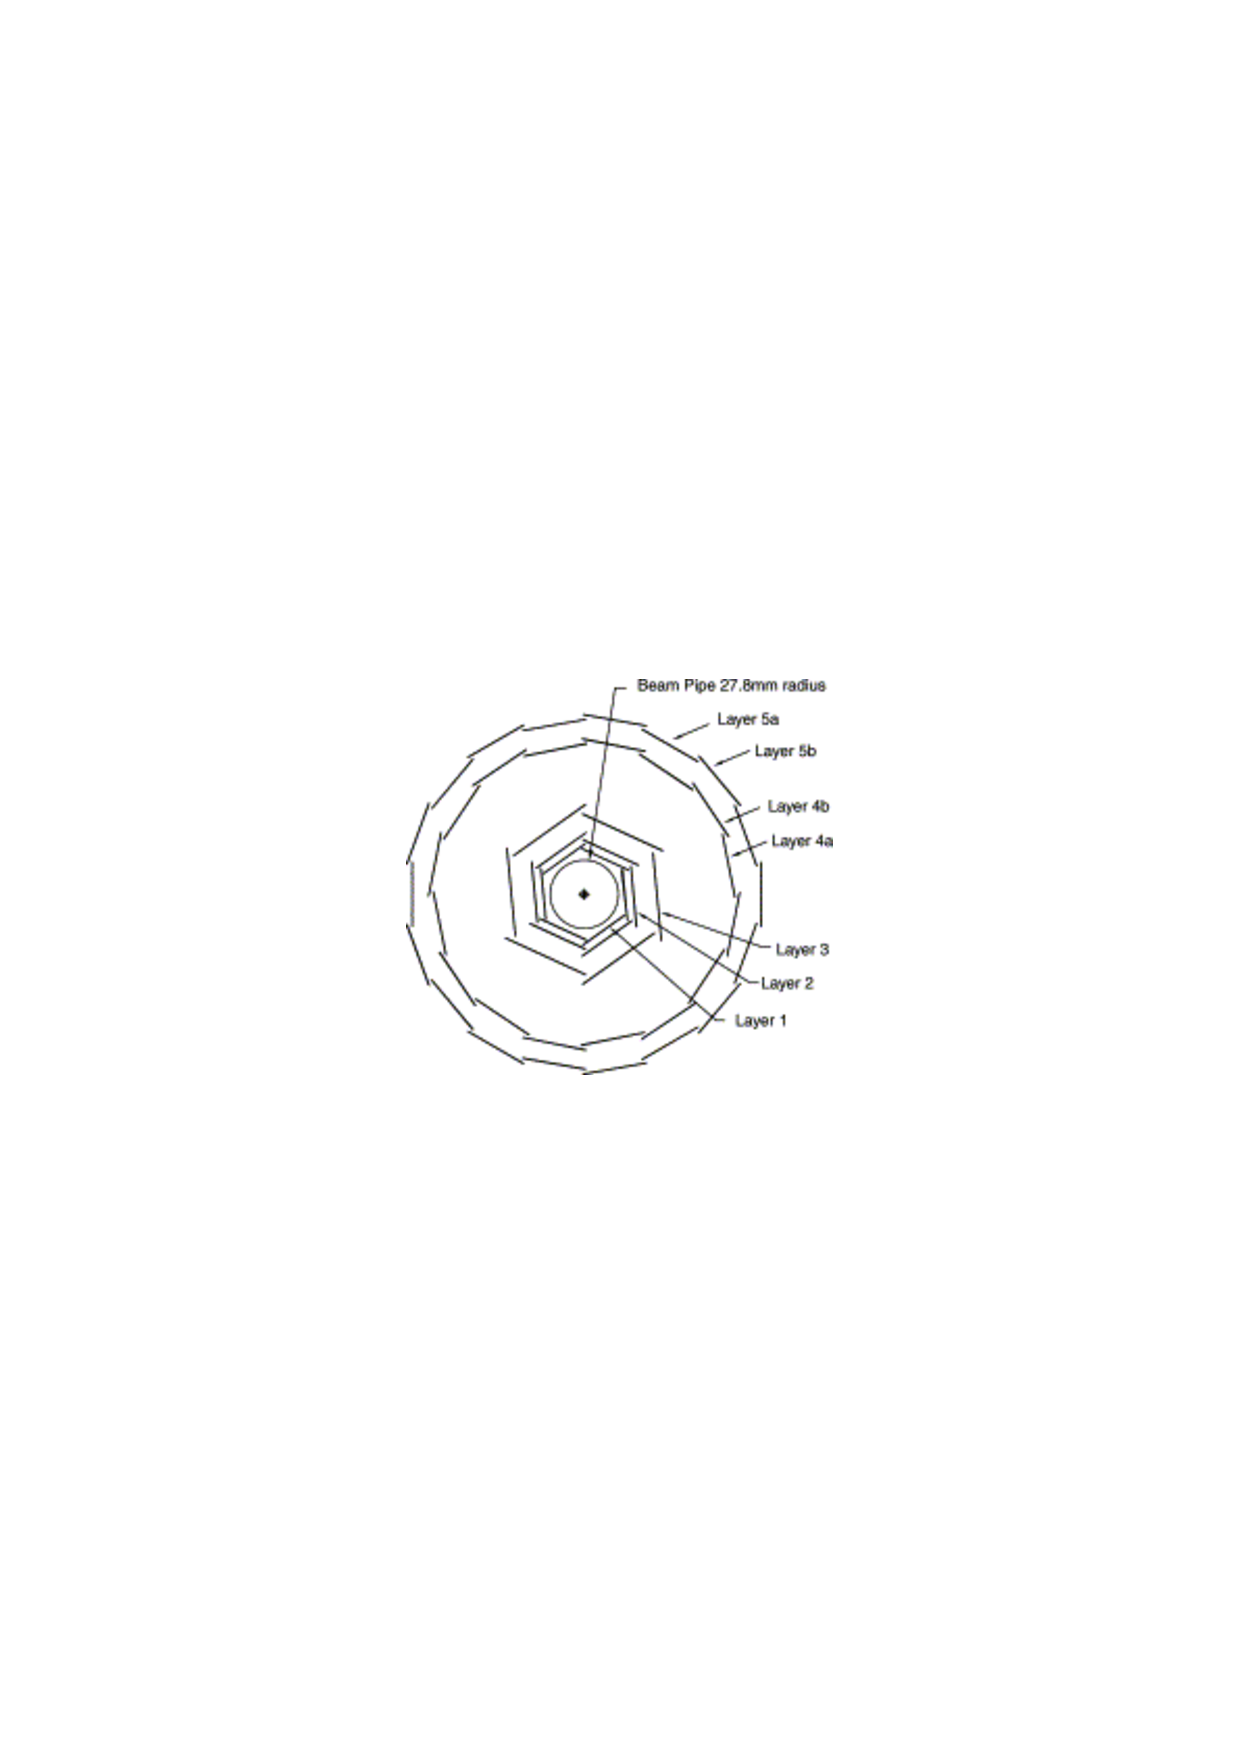
\includegraphics[width=0.45\textwidth]{miniSVT.pdf}
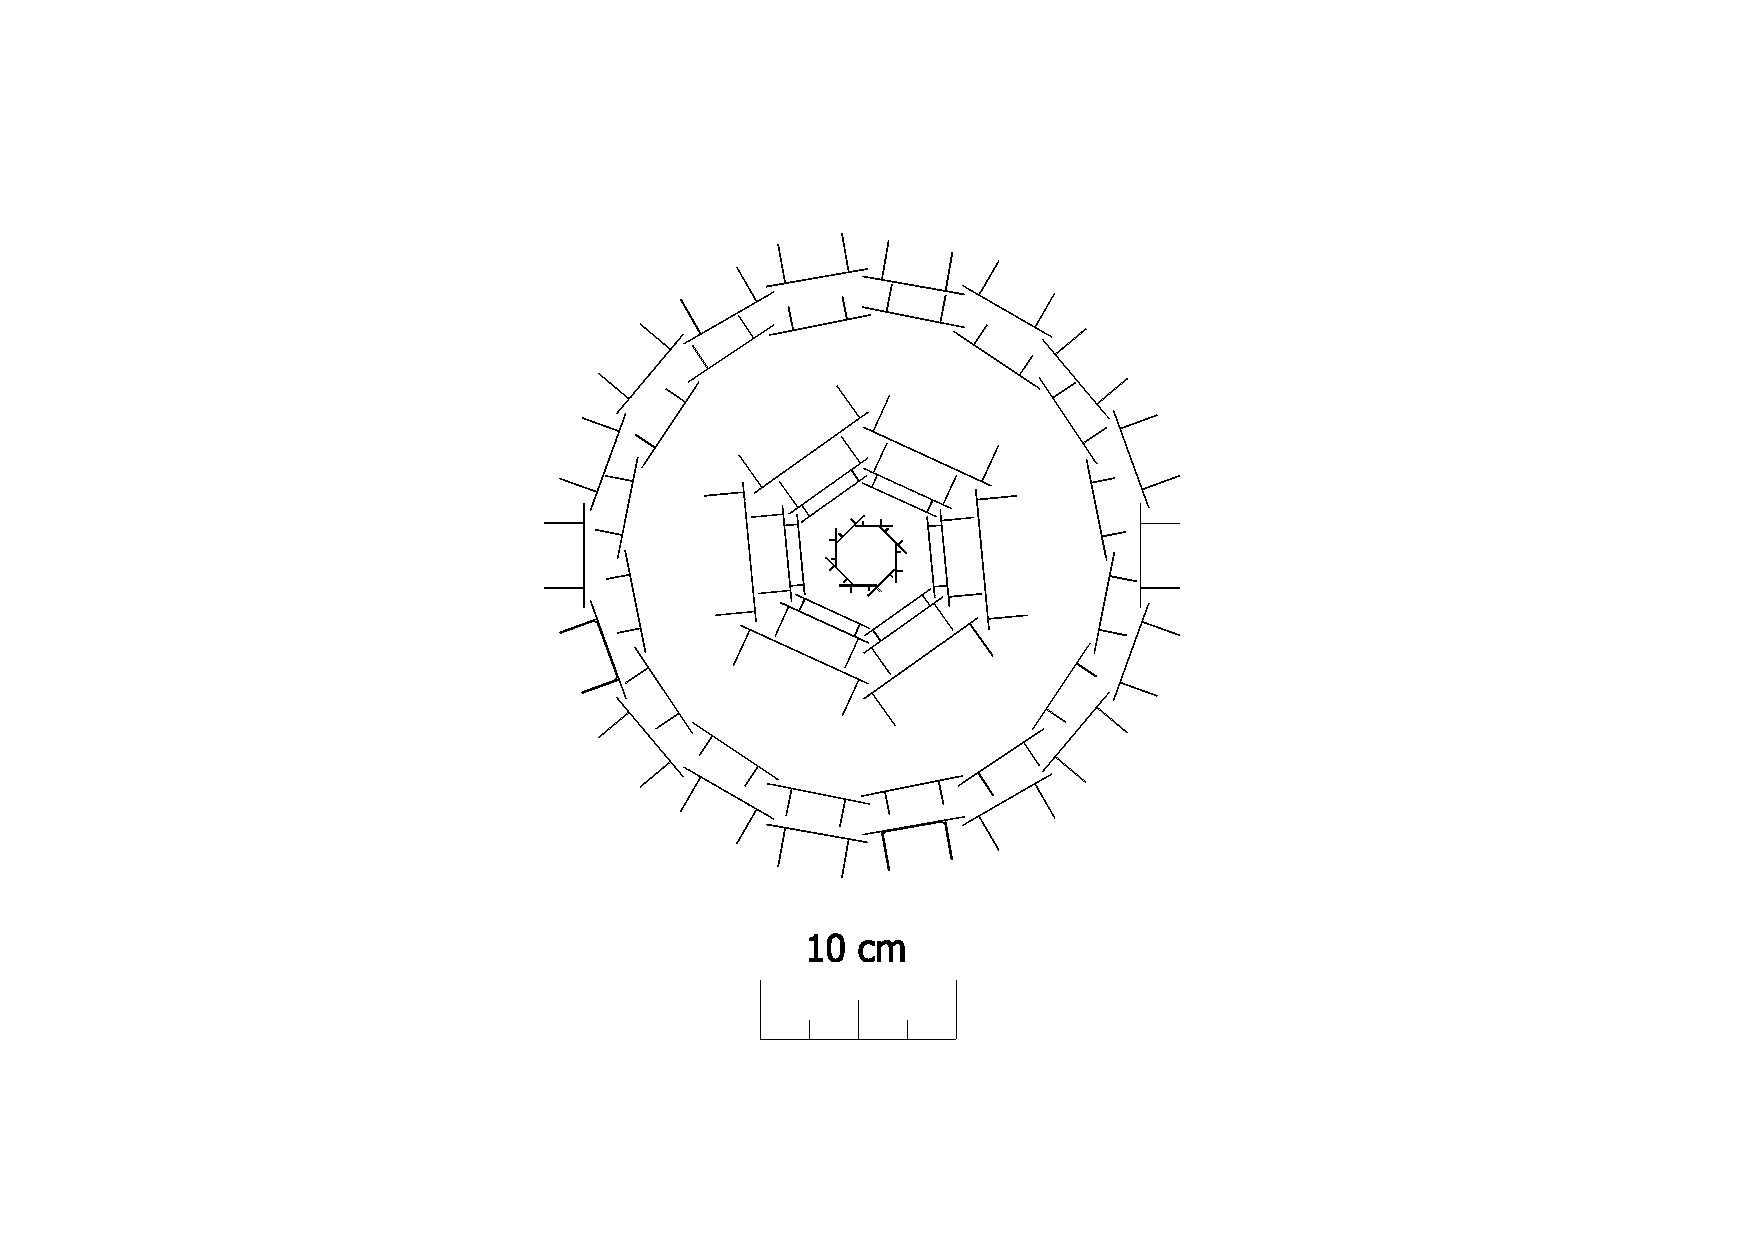
\includegraphics[width=0.45\textwidth]{miniSuperBSVT.pdf}
\caption{\label{fig:svt} (left)Schematic view of \babar\ SVT: tranverse section. (After~\cite{AUBERT20021}) The external radius is 144 mm. (right) Cross section of the SuperB SVT. (After~\cite{Baszczyk:2013xua}) }
\end{figure}


Precise vertex information, primarily extracted from precise position measurements near the 
interaction point (IP) by the SVT  is crucial to the measurement of time-dependent \CP asymmetries 
in \Bz decays, which was the  key element of the SuperB physics program. As in \babar, the SuperB 
had to be able to provide efficient and accurate tracking for  charged particles with transverse 
momenta lower than 100~MeV/c, which cannot reach the tracking Drift Chamber.

SuperB SVT had to be capable of maintaining adequate performance for time-dependent 
measurements
 in the presence of a lower boost of the center-of-mass (CM) frame
($\beta\gamma = 0.24$ compared to $\beta\gamma = 0.55$ of \babar) and much higher background,
mainly related to the increased instantaneous luminosity of about a factor of 100 larger than \babar.

The planned beam pipe featured a reduced radius of about $1.0~\cm$  which allows the positioning of 
Layer0 at
the desired average radius of about $1.5~\cm$. The additional  (with respect to \babar SVT) 
 Layer0 measurement,
along with the low radial material budget of the beam pipe ($0.42\%~X_0$)
and of Layer0 ($0.45\%~X_0$ with the striplet option - see Section~\ref{sec:Striplets}),
was crucial for improving the decay vertex reconstruction of the \B mesons and
 obtaining adequate proper-time resolution for time-dependent \CP violation measurements.

Physics simulations for the $B\to\pip\pim$ decay channel showed that to retain or improve the vertexing performance of the \babar\ SVT in the SuperB environment the following ingredients were necessary: the use of high granularity pixels (50~$\mu$m $\times$50~$\mu$m pitch), going indeed closer to the beam pipe and very low material budget~\cite{RIZZO2010585}. Results are shown in 
Figure~\ref{fig:bpipi}. 

\begin{figure}
\centering
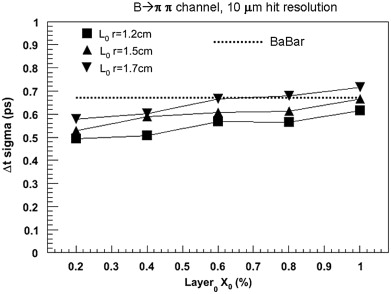
\includegraphics[width=0.45\textwidth]{bpipi}
\caption{\label{fig:bpipi} Resolution on the proper time difference of the two B mesons for the nominal SuperB boost, for different Layer0 radii, as a function of Layer0 thickness (in $X_0$ \%). The BaBar resolution for the same decay channel, is shown with a dashed line. (After~\cite{RIZZO2010585})}
\end{figure}

In summary, for the SuperB physics program a silicon tracker detector was needed with the 
capability to assure a space-point resolution of 10~$\mu$m, with a material budget below 
1\% of $X_0$, able to measure tracks with $p_T$ lower then 100~MeV/c. The real detector 
would have had to withstand a particle rate of 100~MHz/cm$^2$, mainly due to machine 
background.

\subsection{ILC}
\cite{ILCVertexing2007}


\section{The CMOS MAPS Apsel4D}
\label{sec:Apsel4D}

\section{The Striplets Detector}
\label{sec:Striplets}

\section{Discussion of the Performance of SLIM5 Detectors}
\label{sec:SLIM5Results}
A demonstrator was built~\cite{BETTARINI2010942}, it was composed of CMOS MAPS 
 and thin silicon DSSDs and tested it on beam at the T9 facility of the CERN PS. 


\section{Summary}
